\documentclass[a4j,titlepage]{jsarticle}

\usepackage[dvipdfmx]{graphicx,xcolor}
\usepackage[top=20truemm,left=25truemm,right=25truemm]{geometry}
\usepackage{amsmath}
\usepackage{here}
\usepackage{comment}
\usepackage{url}
\usepackage{plistings}
\usepackage{tikz}
\usepackage[framemethod=tikz]{mdframed}

\renewcommand{\lstlistingname}{リスト}

\newcommand{\chuo}[1]{\multicolumn{1}{|c|}{#1}}
\newcommand{\inpt}[1]{\underline{#1}\,\setlength{\fboxsep}{1pt}\fbox{\small ↓}}
\newcommand{\bvec}[1]{\mbox{\boldmath $#1$}}

\lstdefinestyle{python}{
  language=Python,
  basicstyle=\small\ttfamily,
  keywordstyle=\color[HTML]{0000E0},
  stringstyle=\color[HTML]{A31515},
  commentstyle=\upshape\color[HTML]{008000},
  frame=trbl,
  framesep=5pt,
  columns=[l]{fullflexible},
  numbers=left,
  xleftmargin=3zw,
  lineskip=-0.2ex,
  breaklines=true,
  showstringspaces=false,
  tabsize=4,
  keepspaces=true
}

\lstdefinestyle{text}{
  language=,
  basicstyle=\ttfamily,
  frame=trbl,
  framesep=5pt,
  columns=[l]{fullflexible},
  xleftmargin=3zw,
  lineskip=-0.2ex,
  showstringspaces=false,
  tabsize=4,
  keepspaces=true
}

\mdfsetup{
  skipabove=5pt,
  innertopmargin=10pt,
  innerbottommargin=10pt,
  roundcorner=10pt,
  font=\ttfamily
}


\begin{document}


\begin{titlepage}
  \title{\huge{ネットワークプログラミングI\hspace{-.1em}I} \\ \LARGE{---麻雀ゲームの作成---}}
  \author{
    学籍番号:16418 \\ 5年 電子情報工学科 16番 \\ 多田 洋輔 \\ \\
    学籍番号:16426 \\ 5年 電子情報工学科 24番 \\ 福澤 大地
  }
	\date{提出日 : 2020年8月6日}
  \maketitle
\end{titlepage}


\section{作成したプログラム}
オンライン対戦可能な麻雀ゲームを作成した。
ルールはオーソドックスな日本のリーチ麻雀であるが、3人/4人対戦どちらも対応していたり、
AIを交えた対戦が可能であったりと、細かな機能を充実させた。
また、操作はCUIで行うが、OpenCVを用いることで卓上の状態をグラフィカルに表示した。

使用したプログラミング言語は、Python 3.7.4である。


\section{動作説明}
麻雀で行う主な動作について、サーバー側とプレイヤー側でどのような動作をしているかを示す。

\subsection{ポン}
図\ref{fig:pon_server}から図\ref{fig:pon_gui}に打牌時の動作を示す。

\begin{figure}[htbp]
  \centering
  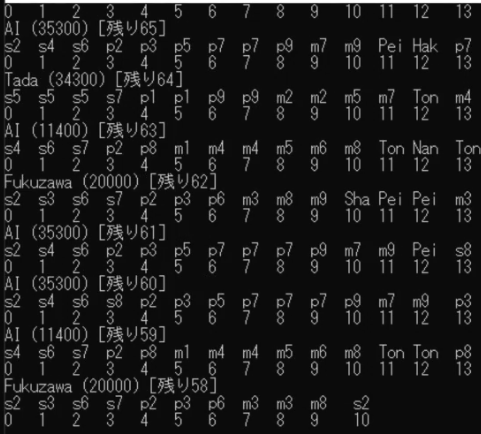
\includegraphics[width = 0.8\linewidth]{images/pon_server.png}
  \caption{ポンの動作(サーバー)}
  \label{fig:pon_server}
\end{figure}

\begin{figure}[htbp]
  \centering
  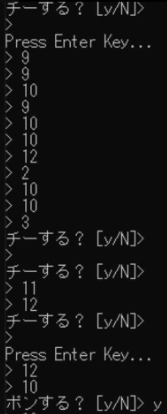
\includegraphics[width = 0.2\linewidth]{images/pon_console.png}
  \caption{ポンの動作(コンソール)}
  \label{fig:pon_console}
\end{figure}

\begin{figure}[htbp]
  \centering
  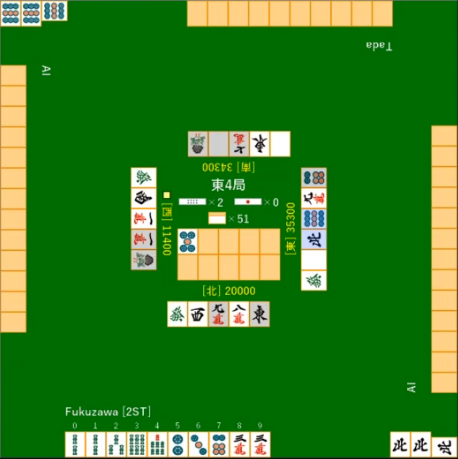
\includegraphics[width = 0.8\linewidth]{images/pon_gui.png}
  \caption{ポンの動作(GUI)}
  \label{fig:pon_gui}
\end{figure}

サーバーではポンをしたプレイヤーの手牌からポンの構成牌がなくなっている。コンソールではポンするかどうかに対し、y(yes)を入力している。これに対しGUIにはポンの様子が表示されている。

\subsection{チー}
図\ref{fig:chi_server}から図\ref{fig:chi_gui}に打牌時の動作を示す。

\begin{figure}[htbp]
  \centering
  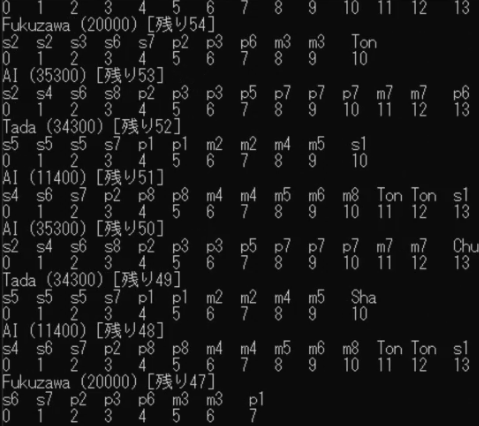
\includegraphics[width = 0.8\linewidth]{images/chi_server.png}
  \caption{チーの動作(サーバー)}
  \label{fig:chi_server}
\end{figure}

\begin{figure}[htbp]
  \centering
  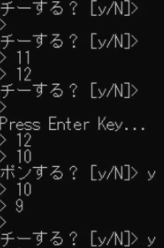
\includegraphics[width = 0.4\linewidth]{images/chi_console.png}
  \caption{チーの動作(コンソール)}
  \label{fig:chi_console}
\end{figure}

\begin{figure}[htbp]
  \centering
  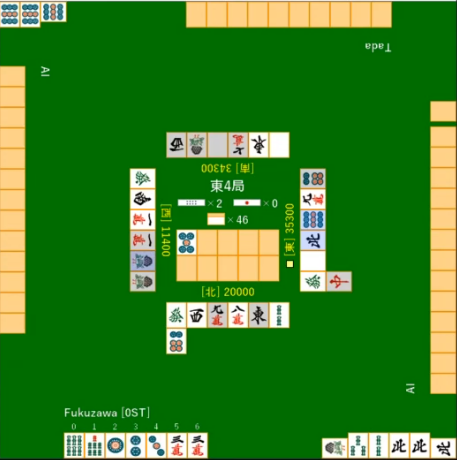
\includegraphics[width = 0.8\linewidth]{images/chi_gui.png}
  \caption{チーの動作(GUI)}
  \label{fig:chi_gui}
\end{figure}

サーバーでは、チーをしたプレイヤーが以前にポンをしていたため、手牌から2鳴き分の構成牌が消えている。コンソールではチーするかどうかに対し、y(yes)を入力している。これに対しGUIにはチーの様子が表示されている。

\subsection{暗カン}
図\ref{fig:ankan_server}から図\ref{fig:ankan_gui}に打牌時の動作を示す。

\begin{figure}[htbp]
  \centering
  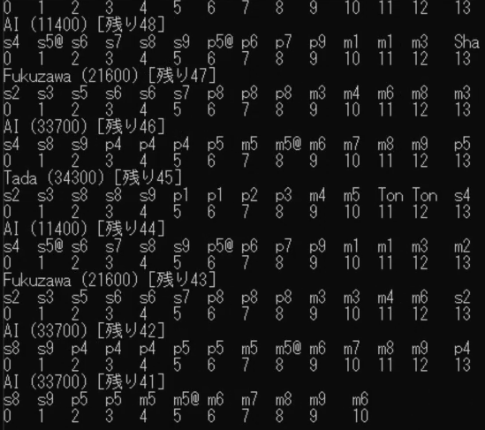
\includegraphics[width = 0.8\linewidth]{images/ankan_server.png}
  \caption{暗カンの動作(サーバー)}
  \label{fig:ankan_server}
\end{figure}

\begin{figure}[htbp]
  \centering
  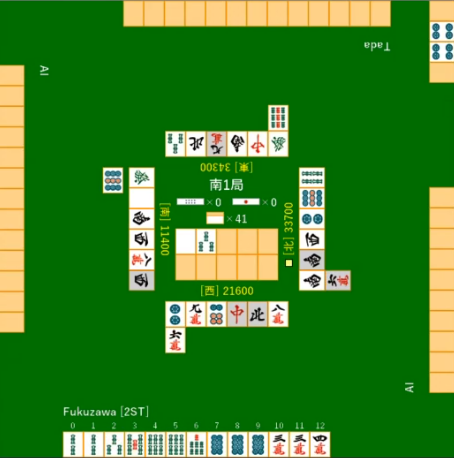
\includegraphics[width = 0.8\linewidth]{images/ankan_gui.png}
  \caption{暗カンの動作(GUI)}
  \label{fig:ankan_gui}
\end{figure}

サーバーでは暗カンをしたプレイヤーの手牌から暗カンに使われた牌が消えている。AIが暗カンをしたためコンソールの表示はないが、GUIには暗カンの様子が表示されている。

\subsection{明カン}
図\ref{fig:minkan_server}から図\ref{fig:minkan_gui}に打牌時の動作を示す。

\begin{figure}[htbp]
  \centering
  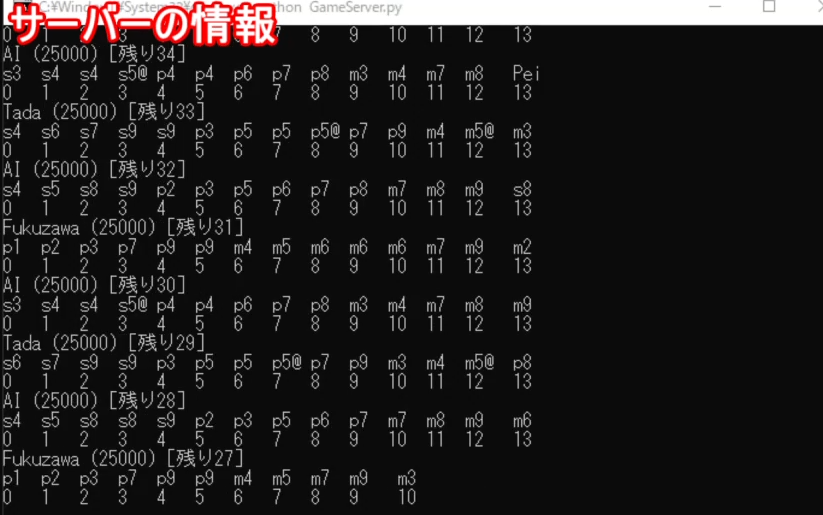
\includegraphics[width = 0.8\linewidth]{images/minkan_server.png}
  \caption{明カンの動作(サーバー)}
  \label{fig:minkan_server}
\end{figure}

\begin{figure}[htbp]
  \centering
  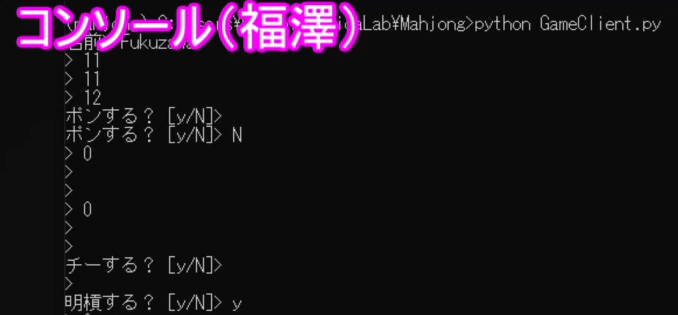
\includegraphics[width = 0.8\linewidth]{images/minkan_console.png}
  \caption{明カンの動作(コンソール)}
  \label{fig:minkan_console}
\end{figure}

\begin{figure}[htbp]
  \centering
  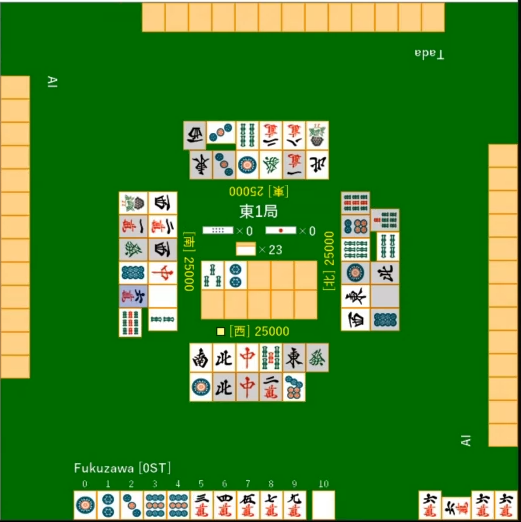
\includegraphics[width = 0.8\linewidth]{images/minkan_gui.png}
  \caption{明カンの動作(GUI)}
  \label{fig:minkan_gui}
\end{figure}

サーバーでは明カンを舌プレイヤーの手牌から明カンに使われた牌が消えている。コンソールでは暗カンするかどうかに対し、y(yes)が入力されている。これに対しGUIには明カンの様子が表示されている。

\subsection{ロン}
図\ref{fig:ron_server}から図\ref{fig:ron_gui}に打牌時の動作を示す。

\begin{figure}[htbp]
  \centering
  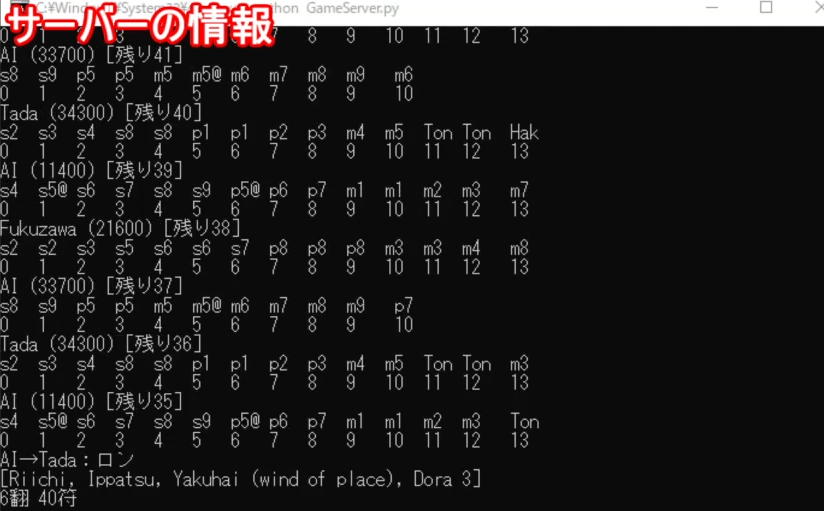
\includegraphics[width = 0.8\linewidth]{images/ron_server.png}
  \caption{ロンの動作(サーバー)}
  \label{fig:ron_server}
\end{figure}

\begin{figure}[htbp]
  \centering
  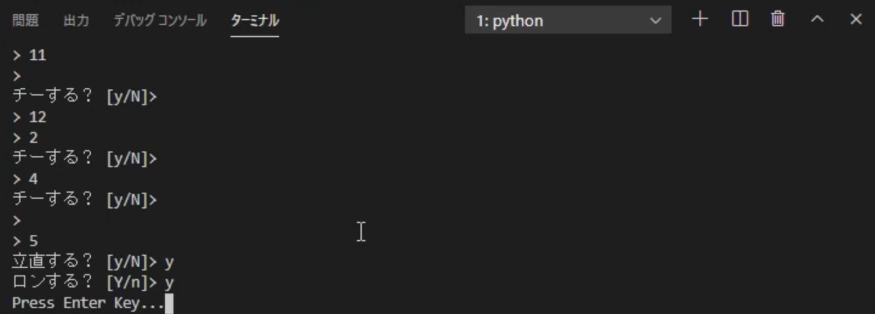
\includegraphics[width = 0.8\linewidth]{images/ron_console.png}
  \caption{ロンの動作(コンソール)}
  \label{fig:ron_console}
\end{figure}

\begin{figure}[htbp]
  \centering
  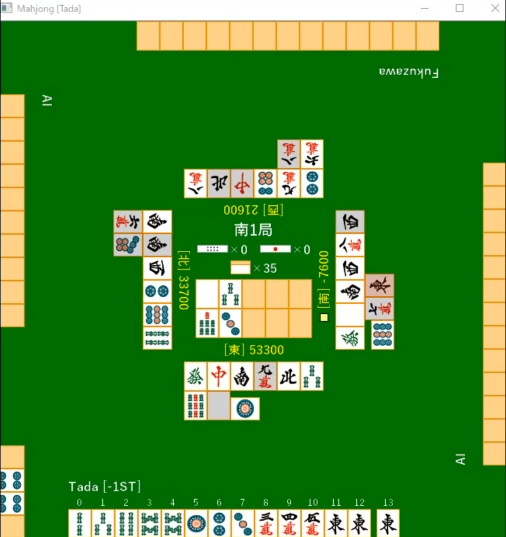
\includegraphics[width = 0.8\linewidth]{images/ron_gui.png}
  \caption{ロンの動作(GUI)}
  \label{fig:ron_gui}
\end{figure}

サーバーではロンに関わったプレイヤーと、役の内容が表示されている。コンソールではロンするかどうかに対しy(yes)が入力されている。これに対しGUIではロンをした牌が赤みがかり、ロンを表現している。

\subsection{ツモ}
図\ref{fig:tsumo_server}から図\ref{fig:tsumo_gui}に打牌時の動作を示す。

\begin{figure}[htbp]
  \centering
  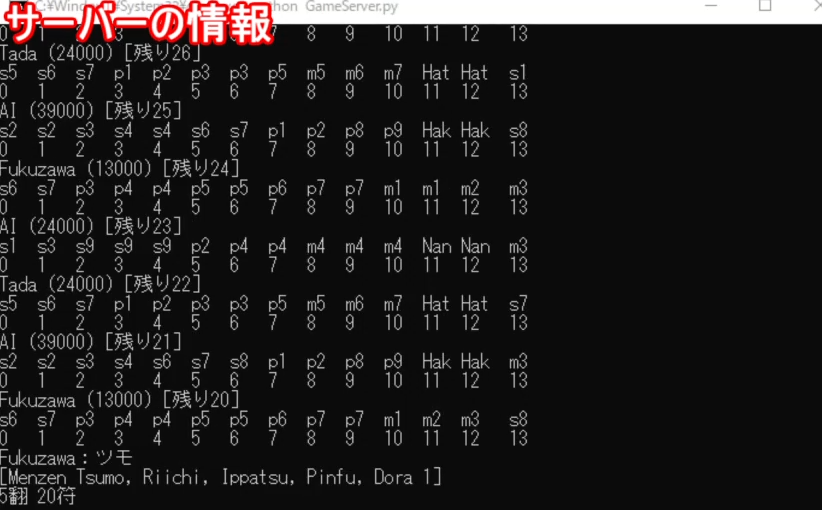
\includegraphics[width = 0.8\linewidth]{images/tsumo_server.png}
  \caption{ツモの動作(サーバー)}
  \label{fig:tsumo_server}
\end{figure}

\begin{figure}[htbp]
  \centering
  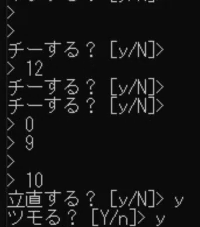
\includegraphics[width = 0.5\linewidth]{images/tsumo_console.png}
  \caption{ツモの動作(コンソール)}
  \label{fig:tsumo_console}
\end{figure}

\begin{figure}[htbp]
  \centering
  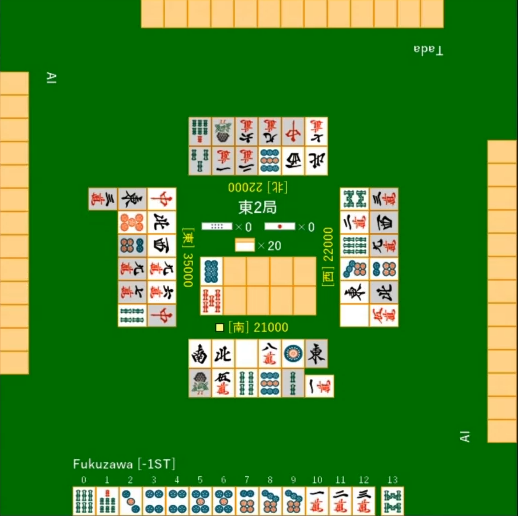
\includegraphics[width = 0.8\linewidth]{images/tsumo_gui.png}
  \caption{ツモの動作(GUI)}
  \label{fig:tsumo_gui}
\end{figure}

サーバーではツモをしたプレイヤーと、役の内容が表示されている。コンソールではツモをするかどうかに対しy(yes)を入力している。これに対しGUIにはツモった牌を表示している。

\subsection{流局}
図\ref{fig:ryukyoku_server}から図\ref{fig:ryukyoku_gui}に打牌時の動作を示す。

\begin{figure}[htbp]
  \centering
  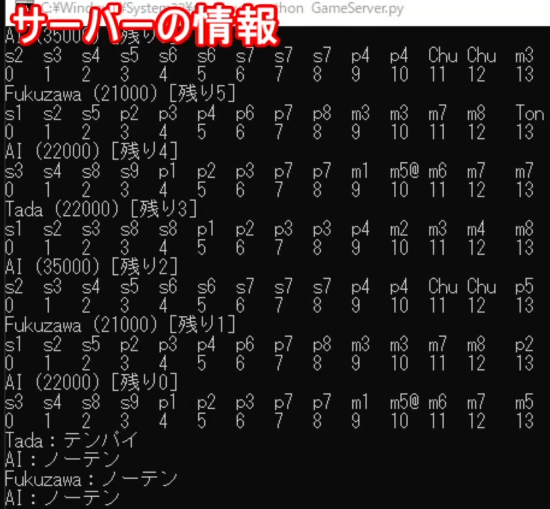
\includegraphics[width = 0.7\linewidth]{images/ryukyoku_server.png}
  \caption{流局の動作(サーバー)}
  \label{fig:ryukyoku_server}
\end{figure}

\begin{figure}[htbp]
  \centering
  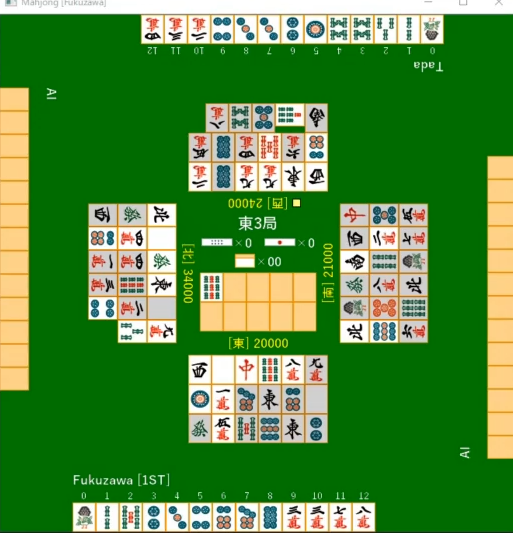
\includegraphics[width = 0.8\linewidth]{images/ryukyoku_gui.png}
  \caption{流局の動作(GUI)}
  \label{fig:ryukyoku_gui}
\end{figure}

サーバーでは各プレイヤーのテンパイ状況を表示している。これに対しGUIではテンパイのプレイヤーの手牌が倒されて表示されている。

\newpage
\section{クラス図}
本システムのクラス図を図\ref{fig:class}に示す。
詳細な説明は省略するが、ゲームの進行を表す\texttt{Game}クラスを\texttt{GameServer}クラスに継承し、
ソケット通信でオンライン対戦を行う機能をオーバーライドしている。

\begin{figure}[p]
  \centering
  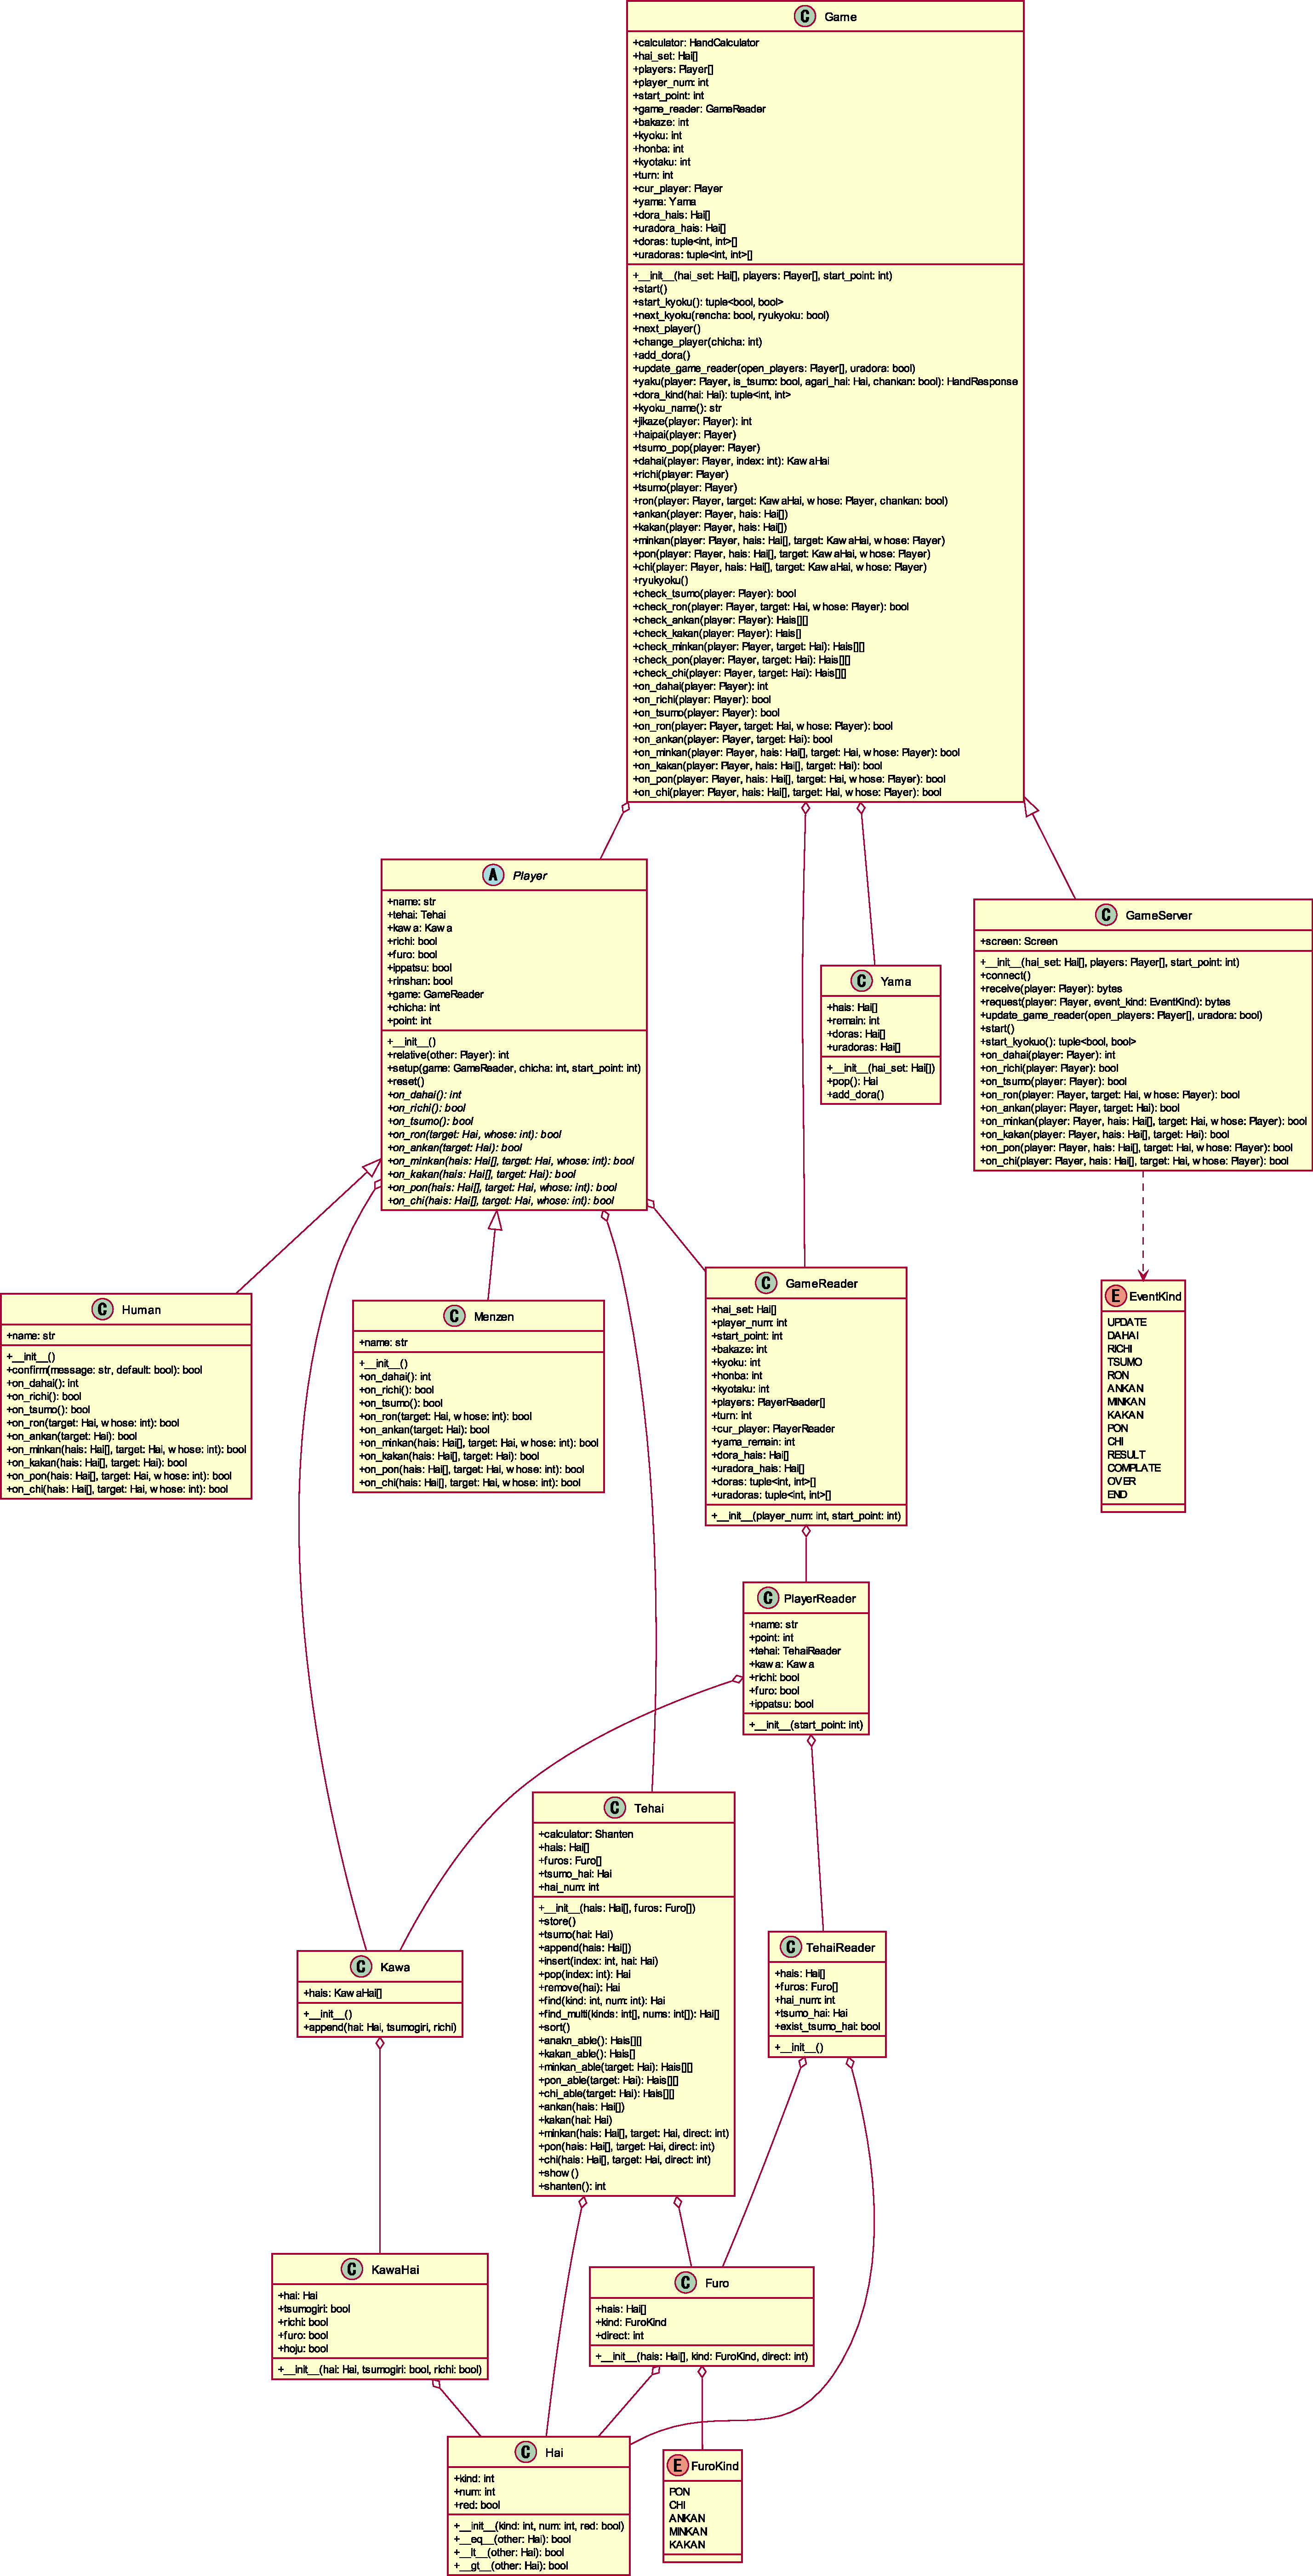
\includegraphics[height=23cm]{images/mahjong.pdf}
  \caption{クラス図}
  \label{fig:class}
\end{figure}

\section{ファイル構造}
本システムのファイル構造を図\ref{fig:file}に示す。
\texttt{GameServer.py}はサーバーサイドのプログラム、
\texttt{GameClient.py}はクライアントサイドのプログラムである。
その他の麻雀システムのプログラムは\texttt{mjgame}フォルダ内にまとめられている。

\begin{figure}[H]
  \centering
  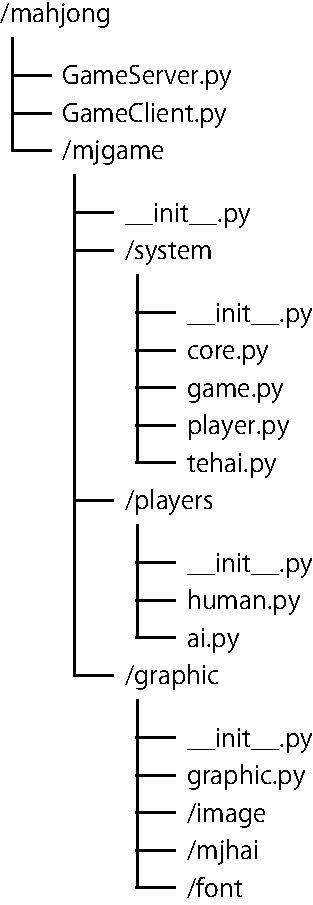
\includegraphics[height=13cm]{images/file.pdf}
  \caption{ファイル構造}
  \label{fig:file}
\end{figure}

\newpage
\section{プログラムリスト}
サーバーサイドのプログラムをリスト\ref{lst:GameServer}に、
クライアントサイドのプログラムをリスト\ref{lst:GameClient}に示す。
その他の麻雀システムのプログラムはリスト\ref{lst:mjgame}--\ref{lst:graphic}に示す。

\lstinputlisting[style=python,caption=GameServer.py,label=lst:GameServer]{mahjong/GameServer.py}

\lstinputlisting[style=python,caption=GameClient.py,label=lst:GameClient]{mahjong/GameClient.py}

\lstinputlisting[style=python,caption=mjgame/\_\_init\_\_.py,label=lst:mjgame]{mahjong/mjgame/__init__.py}

\lstinputlisting[style=python,caption=mjgame/system/\_\_init\_\_.py,label=lst:system]{mahjong/mjgame/system/__init__.py}

\lstinputlisting[style=python,caption=mjgame/system/core.py,label=lst:core]{mahjong/mjgame/system/core.py}

\lstinputlisting[style=python,caption=mjgame/system/game.py,label=lst:game]{mahjong/mjgame/system/game.py}

\lstinputlisting[style=python,caption=mjgame/system/player.py,label=lst:player]{mahjong/mjgame/system/player.py}

\lstinputlisting[style=python,caption=mjgame/system/tehai.py,label=lst:tehai]{mahjong/mjgame/system/tehai.py}

\lstinputlisting[style=python,caption=mjgame/players/\_\_init\_\_.py,label=lst:players]{mahjong/mjgame/players/__init__.py}

\lstinputlisting[style=python,caption=mjgame/players/human.py,label=lst:human]{mahjong/mjgame/players/human.py}

\lstinputlisting[style=python,caption=mjgame/players/ai.py,label=lst:ai]{mahjong/mjgame/players/ai.py}

\lstinputlisting[style=python,caption=mjgame/graphic/\_\_init\_\_.py,label=lst:graphici]{mahjong/mjgame/graphic/__init__.py}

\lstinputlisting[style=python,caption=mjgame/graphic/graphic.py,label=lst:graphic]{mahjong/mjgame/graphic/graphic.py}


\end{document}
